\documentclass[12pt,letterpaper]{article}

\PassOptionsToPackage{hyphens}{url}
\usepackage[pdftex, bookmarksopen=true, bookmarksnumbered=true,
pdfstartview=FitH, breaklinks=true, urlbordercolor={0 1 0}, citebordercolor={0 0 1}]{hyperref}

% === MARGINS ===
\addtolength{\hoffset}{-0.75in} \addtolength{\voffset}{-1.25in}
\addtolength{\textwidth}{1.5in} \addtolength{\textheight}{2.25in}

% == ENVS ==
\newenvironment{tightcenter}{%
  \setlength\topsep{0pt}
  \setlength\parskip{0pt}
  \begin{center}
}{
  \end{center}
}

% == PACKS ==
\usepackage{color,soul}
\usepackage{graphicx}
\usepackage{calc} % To scale \pagewidth with \real{float}
\usepackage{pgfplots} % To draw histogram
\pgfplotsset{compat=1.17} % request specific version of pgfplots
\usepackage{calc} % to use \real for text -> numeric
\usepackage{pgf} % to store numeric variables
\usepackage{subcaption} % to place two figures horizontally
\usepackage{caption} % to refer subfigure
\renewcommand{\thesubfigure}{(\alph{subfigure})}
\captionsetup[sub]{labelformat=simple}

\usepackage{tikz}
\usetikzlibrary{automata,positioning}
\usetikzlibrary{arrows.meta, positioning, automata}
\tikzset{
  font={\fontsize{10pt}{0}\selectfont}}
\usepackage{forest}
\tikzset{
  Decision/.style = {%
    draw,
    line width=1.4pt
  },
  Lottery/.style = {%
    draw,
    line width=1.4pt
  },
  Outcome/.style = {%
    circle,
    minimum width=3pt,
    fill,
    inner sep=0pt
  }
}
\usepackage{csquotes}
\usepackage{lipsum}
\usetikzlibrary{arrows.meta,automata,positioning} % to draw directed-weighted-graph


\usepackage{amsmath, amssymb, latexsym} % NN
\usepackage{tikz}% NN
\usetikzlibrary{decorations.pathreplacing}% NN
\usetikzlibrary{fadings}% NN

% == BIBS ==
\usepackage{natbib}
\bibliographystyle{apsr}

% == SPACES == 

% == CMMDS ==
\newcommand{\tit}{
\bf 
Mapping Regulatory Network of WTO Dispute Settlement Body Using Deep Learning
}
\newcommand\spacingset[1]{\renewcommand{\baselinestretch}
{#1}\small\normalsize}

% == VARS == 
\pgfmathsetmacro{\heatmap}{1}

% == START (PageCounter, Mode)
\begin{document}

\spacingset{1.25}

\setcounter{page}{0}
\vspace{-.1in}

% == TITLE (includes DraftDate)
{\title{
    \tit
  }
  \author{Suyeol Yun
  }
  \maketitle
}

\thispagestyle{empty}
\vspace{-.1in}

\begin{abstract}
  \lipsum[1]
\end{abstract}

\spacingset{1.5} % gives a slightly more margin between abstract and introduction

% \section{Tree of Contents}
% \begin{forest}
  for tree={
  % grow=-1,
  Decision,
  }
  [Introduction
    [How WTO works]
    [Complexity in Legal Citation
        [Origin of Complexity
            [Strategic Consideration]
        ]
        [Importance of Understanding this Complexity
          [Difficult to Map this Complexity]
        ]
    ]
  ]
\end{forest}


\section{Introduction}

The Dispute Settlement Body (DSB) of 
the World Trade Organization (WTO) deals 
with trade disputes between WTO members.
WTO members can file a lawsuit in WTO DSB to 
claim their impaired benifit related to the WTO agreements as a result of possible illegal action of the other member's trade policy.
Then a judicial body, \textit{Panel} or \textit{Appellate Body}, %``Panel'' or ``Appellate Body'', 
adjudicates the dispute and submits a report in which it expresses
its judicial opinion as to whether the challenged 
trade policy is inconsistent to the rules of the WTO or not \citep{world2017handbook}.

 
% References
% https://www.wto.org/english/tratop_e/dispu_e/disp_settlement_cbt_e/c3s3p1_e.htm


A lawsuit tends to cite multiple rules of the WTO agreement because a trade policy is usually pretty much complicated
and one simple rule can't cover the characteristics of the trade policy at issue \citep{palmeter2004dispute}.
For example, the United States enacted \textit{Continued Dumping and Subsidy Act of 2000 (Byrd Amendment)} that distributes
the collected anti-dumping duties to its affected domestic producers and this act was challenged with multiple rules of the WTO agreement,
such as \textit{Anti-dumping} and \textit{Subsidy}, because
this distribution could constitute a illegal subsidy prohibited
in the rules of the WTO agreement although it's mainly related to the rules of the anti-dumping \citep{cdsoa}.
 
% Todos:
% - How to cite us laws? Byrd amendment


Moreover, legal citation becomes even more complicated because members cite the 
rules of the WTO agreement strategically. For example,
members cite different rules of the WTO agreement to limit or to encourage 
the third party participation because the third party 
participation can lead to eary settlement of the dispute without continuos 
legal battle and vice versa  \cite{who_gets}.
As WTO sets multiple principles to regulate the world trade system, 
such as \textit{Market Acceess} (across borders), 
\textit{Non-discrimination} (between members 
or between domestic products and imported products) 
and \textit{Transparency} (in publication and maintaining 
of each member's internal regulations), 
it's intellectually intriguing 
to understand how regulatory system of WTO DSB
is structured to achieve these core principles.
By understanding this structure, 
we can improve WTO system more efficiently to adopt to constantly 
changing circumstances of world trade
\citep{FREDEBEULKREIN1999625, shaffer_2004, 10.1093/jiel/jgm028}.




However, it is extremely difficult to 
visually map how regulatory power of 
WTO DSB is organized to acheive 
those core principles. 
As explained above, 
this is because each citation is closely related 
to composite characteristics 
of each trade policy and also 
it requires to generalize those strategic 
citations which are limited 
to each member's special interest 
rather than explaining the 
regulatory power of WTO DSB in general. 


\begin{figure}[ht]
    \[\text{Network of legal articles of WTO agreements is defined as}\] %\textit{directed weighted graph}}  G = (V, E, w) \]
    \[ \textit{directed weighted graph }G = (V, E, W) \]
    \[\text{ where \textit{vertex set} } V = \{v \mid v\text{ is a legal article of WTO agreement}\}  \text{ , } \]
    \[\text{ \textit{set of directed edges }}\vec{E} = \{(v_i, v_j) \mid (v_i, v_j)\in V \times V)\} \text{ and } \]
    \[w : V \times V \to \Bbb R_{+} \text{ } s.t. \text{ } w(v_j, v_j) = 0 \text{ and } \sum_{v_i\in V}{w(v_i, v_j)} = 1 \text{  } \forall v_j \in V \]%\text{ and }\]
    \[\text{Then define \textit{edge weight matrix }}W=(w_{ij}) \in \Bbb{R_{+}}^{|V| \times |V|} \text{ } s.t. \text{ } w_{ij} = w(v_i, v_j) \] % \text{ } s.t. \text{ } w_{ii} = 0 \text{ and } \sum_{v_j\in V}{w_{ji}} = 1 \text{  } \forall v_i \in V \] %\text{ } s.t. \text{ } w_{ij} = w(v_i, v_j)\]
    % \[w_{ij} \text{ notates the weight of a directed edge from } v_i \text{ to } v_j \text{ and }  \]
    \[(W \text{ is more formally called \textit{weighted adjancency matrix}})\]
    % \[w_{ij} \text{ represents a directed edge weight from source node $v_i$ to $v_j$} \text{ and }\]
    % \[w_{ij} \text{ is interpreted as conditional probability P(v_j|v_i)}\]
    % \[\text{ where a source node $v_i$ clarifies the meaning of the target node $v_j$}\]
    % \[w : V \times V \to \Bbb R_{+} \text{ } s.t. \text{ } w(v_i, v_i) = 0 \text{ and } \sum_{v_j\in V}{w(v_i, v_j)} = 1 \text{  } \forall v_i \in V \]%\text{ and }\]
    % \[\text{ Then define \textit{edge weight matrix} } W=(w_{ij}) \in \Bbb{R}^{|V| \times |V|} \text{ } s.t. \text{ } w_{ij} = w(v_i, v_j)\]
    % \[\text{ This paper assumes there exists } W^{*}=(w^{*}_{ij}) \in \Bbb{R}^{|V| \times |V|} \text{ } s.t. \text{ } w_{ij} = w(v_i, v_j)\]
    % \[\text{(}G\text{ is simply called \textit{directed weighted graph)}}\]
    \caption{\textbf{Formal Definition of Network of Legal Articles of WTO agreements: }I define network of legal articles of WTO agreements
        as a directed weighted graph where the sum of all weights coming into a node sum up to 1. $w_{ij}$ is interpreted as conditional probability $P(v_j|v_i)$ how probably a source node $v_i$ clarifies the meaning of the target node $v_j$ compared to other source nodes as illustrated in Figure \ref{fig:def-example}}
    \label{fig:def}
\end{figure}

% % == DEF EXAMPLE == 
\begin{figure}[]
    \captionsetup[subfigure]{justification=centering}
    \begin{subfigure}[b]{1\textwidth}
        \centering{
                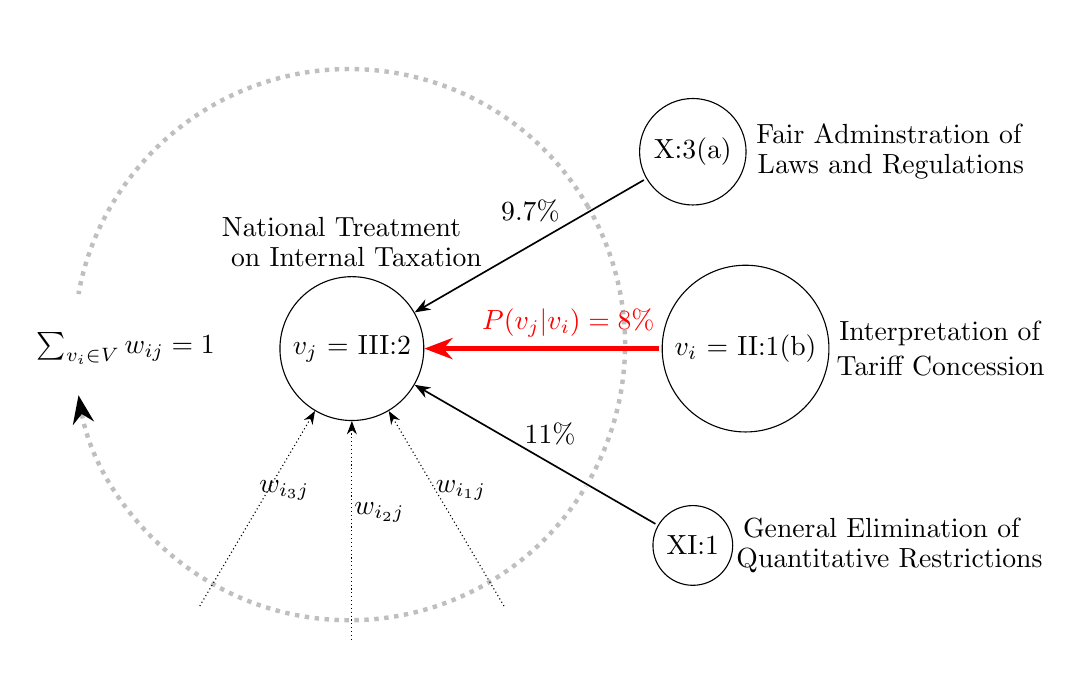
\begin{tikzpicture}[
        >={Stealth[color=black]}
        ,shorten >=1pt,node distance=2cm
        ,on grid,initial/.style={}
        ,every label/.style={align=left}
        ]
        \linespread{2}
        \node[state, label=above:{National Treatment \\[1mm] \hspace{0mm} on Internal Taxation}] (T1) at (10, 0) {$v_j$ = III:2};

        \node[text width=5cm] at (8.5,0)
        {$\sum_{v_i\in V}{w_{ij}} = 1$};

        \draw[ultra thick, gray!50, dotted, ->] (13,1.8) arc (30:-170:3.5);
        \draw[ultra thick, gray!50, dotted, -] (13,1.8) arc (30:170:3.5);

        \node[state, label=right:{Interpretation of \\[1mm] \hspace{-1.5mm} Tariff Concession}] at ([shift=({0:5 cm})]T1) (T2) {$v_i$ = II:1(b)};
        \node[state, label=right:{General Elimination of \\[1mm] \hspace{-2mm} Quantitative Restrictions}] at ([shift=({-30:5 cm})]T1) (T3) {XI:1};
        \node[state, label=right:{Fair Adminstration of \\[1mm] \hspace{-1mm} Laws and Regulations}] at ([shift=({30:5 cm})]T1) (T4) {X:3(a)};
        
        \draw[red,arrows={[red]<-}, ultra thick] node[above, xshift=12.75cm] {$P(v_j|v_i) = 8\%$} (T1) -- (T2);

        \begin{scope}[every edge/.append style={<-}] % for directed edge, change "style={->, double=black, draw=white}]"
            \path
            % (T1) edge[red, ultra thick] node[above] {$0.092$} (T2)
            (T1) edge[double=black, draw=white] node[above, xshift=5pt] {$11\%$} (T3)
            (T1) edge[double=black, draw=white] node[above, yshift=5pt] {$9.7\%$} (T4);

            \path[->] (T1) edge[thin,<-,densely dotted] node[above, xshift=5pt] {$w_{i_{1}j}$} +(1.95,-3.3);
            \path[->] (T1) edge[thin,<-,densely dotted] node[above, xshift=10pt] {$w_{i_{2}j}$} +(0,-3.75);
            \path[->] (T1) edge[thin,<-,densely dotted] node[above, xshift=10pt] {$w_{i_{3}j}$} +(-1.95,-3.3);
        \end{scope}

    \end{tikzpicture}

% \begin{figure}[ht]
%     \centering
    
%     \caption{\textbf{Example of Network of Legal Articles of WTO agreements: }}
%     \label{fig:def-example}
% \end{figure}

        }
        \caption{\textbf{Illustrated edge weights of a target node Article III:2}}
        \label{subfig:a:art2b}
    \end{subfigure}
    \vfill
    \begin{subfigure}[b]{1\textwidth}
        \centering{
            \begin{displayquote}[][]
    \begin{center}
    \end{center}
  
    \begin{displayquote}[][]
    ``The dictionary definition of the noun `excess' is `[t]he amount by which one number
        or quantity exceeds another'. More specifically, `in excess of' means `more than'. Thus,
        as a textual matter, a particular number or quantity is `in excess of' another number
        or quantity if it is greater, regardless of the extent to which it is greater. 
      \textbf{\textit{Looking at the context of Article II:1(b), first sentence, we note that Article III:2, first
      sentence, of the GATT 1994 is cast in very similar terms and in fact uses the phrase
      `in excess of'}}:\\
        \begin{displayquote}
        The products of the territory of any contracting party imported into the
      territory of any other contracting party shall not be subject … to internal
      taxes or other internal charges of any kind in excess of those applied … to
      like domestic products \ldots
        \end{displayquote}   
    \end{displayquote}  
  \end{displayquote}

        }
        \centering
        \caption{\textbf{Jurisprudence of Panel in \textit{Russia – Tariff Treatment} case:} \\ Panel clarifies the point that the meaning of the term \textit{`in excess of'} in Article II:1(b) \\ clarifies the meaning of the same phrase in Article III:2.}
        \label{subfig:a:condprob}
    \end{subfigure}
    \caption{\textbf{Illustration of Network of Legal Articles of WTO agreements: }Every directed edge weight $w_{ij}$ is interpreted as the conditional probability $P(v_j|v_i)$ of how probably a source node $v_i$ constitutes a legal context to clarify the meaning of the target node $v_j$ among all other source nodes $v\in V \setminus \{v_i, v_{j}\}$. Above subfigure (a) represents how jurisprudence of \textit{Panel} stated in (b) is represented as an edge weight where the source node Article II:1(b) constitutes the legal context of the target node Article III:2 regarding how to interpret its term \textit{`in exccess of'} with the $8\%$ of importance compared to other possible source articles.}
    \label{fig:def-example}
\end{figure}

\begin{displayquote}[][]
  \begin{center}
    Article 7\\
    Terms of Reference of Panels
  \end{center}

  1. Panels shall have the following terms of reference unless the parties to the dispute
  agree otherwise within 20 days from the establishment of the panel:

  \begin{displayquote}[][]

    ``To examine, in the light of {\bf the relevant provisions} in (name of the covered
    agreement(s) cited by the parties to the dispute), the matter referred to the DSB by
    (name of party) in document … and to make such findings as will assist the DSB in
    making the recommendations or in giving the rulings provided for in that/those
    agreement(s).''
      
  \end{displayquote}

  2. Panels shall address {\bf the relevant provisions} in any covered agreement or agreements
  cited by the parties to the dispute.

  \ldots
\end{displayquote}


\begin{figure}[]
    \begin{center}
        Article I
    \end{center}
    \begin{center}
        \textit{General Most-Favoured-Nation Treatment}
    \end{center}
    1. With respect to customs duties and charges of any kind imposed on or in connection
    with importation or exportation or imposed on the international transfer of payments for
    imports or exports, and with respect to the method of levying such duties and charges, and
    with respect to all rules and formalities in connection with importation and exportation, and
    with respect to all matters referred to in paragraphs 2 and 4 of Article III, any advantage,
    favour, privilege or immunity granted by any contracting party to any product originating in
    or destined for any other country shall be accorded immediately and unconditionally to the
    like product originating in or destined for the territories of all other contracting parties...
    \caption{\textbf{Example of a legal article of the WTO agreements:} Article I:1 of General Agreement on Tariffs and Trade 1994 that prohibits the discrimination between members of WTO.}
    \label{fig:gatt_art1}
\end{figure}


To train this neural network, this paper collected textual description of trade policy 
that led to the dispute and articles of the WTO agreement cited for each dispute
case requested to the WTO DSB 
from 1995 to 2018 (\hyperref[sub:cited-articles-table]{Total $143$ cases. \textit{Check} the list in Appendix A.2}).
Using this collected data, I trained the neural network by enforcing the neural network to answer correctly 
whether a given article of the WTO agreements
can be cited for the given textual description of 
trade policy that led to the dispute (\textit{See} Figure \ref{fig:design-of-nn} and Figure \ref{fig:def:io:nn}).
% After finish training, I collected all the predictions from the trained neural network (Figure \ref{predidction_matrix})
% and fitted a best network of legal articles of the WTO agreement
% using this collection of answers.
After training, I fitted a set of directed edge weight $W^*$ that 
best explains the variance of each article's citability predicted by the trained deep neural network using a ensemble of random forests \citep{genie3}. 

%for given $V$, $E$ % and collection of answers from the trained neural network (Figure \ref{predidction_matrix}) 
%which is widely used in the biomedical engineering to reconstruct gene regulatory networks.\footnote{Anaology of international normative system to genetics maybe natural because gene expressions (achieving main principles of WTO) are governed by complex interaction between multiple regulatory proteins (interaction between legal articles of WTO). Similar notion is adopted in \cite{gene_analogy} to explain the the evolution of norm of transparency in international security.}

To check whether this fitted network of articles of the WTO agreements $G^*$ = ($V$, $E$, $W^*$) maps the regulatory system of WTO DSB properly, this paper
compares the fitted network $G^*$ with the jurisprudence of WTO DSB made by \textit{Panel} and \textit{Appellate Body}. 
This comparison reveals that the fitted network $G^*$ captures the interaction between the articles of WTO agreements
similarly with the jurisprudence of \textit{Panel} and \textit{the Appellate Body}. This similarity guarantees that the fitted network $G^*$ closely maps the regulatory system of WTO DSB since only these two judicial bodies 
can authoritatively consitute the jurisprudence over how rules of WTO agreements are working together 
to achieve the main principles of WTO.

% Morover, this paper justifies the use of textual information inside the textual description of the dispute and legal article by showing that simply using the co-citation pattern between articles of the WTO disputes can't qualitatively fit the $G^*$ (\textit{See} Figure \ref{fig:adj} and Figure \ref{}). 
% Upon this necessity of using the textual information, this paper also justifies the use of neural network that is computationally intensive since it's generally known that proper design of neural network is able to effectively extract information from the textual content.

% Finally, I will explain how this fitting of network of legal articles can contribute to the current study of international normative system.

% \begin{itemize}
%     \item It shows that the result neural network well match with the result of main two judicial bodies.
% \end{itemize}


% == THREE SUBSYSTEM == 
\begin{figure}
  \centering{
    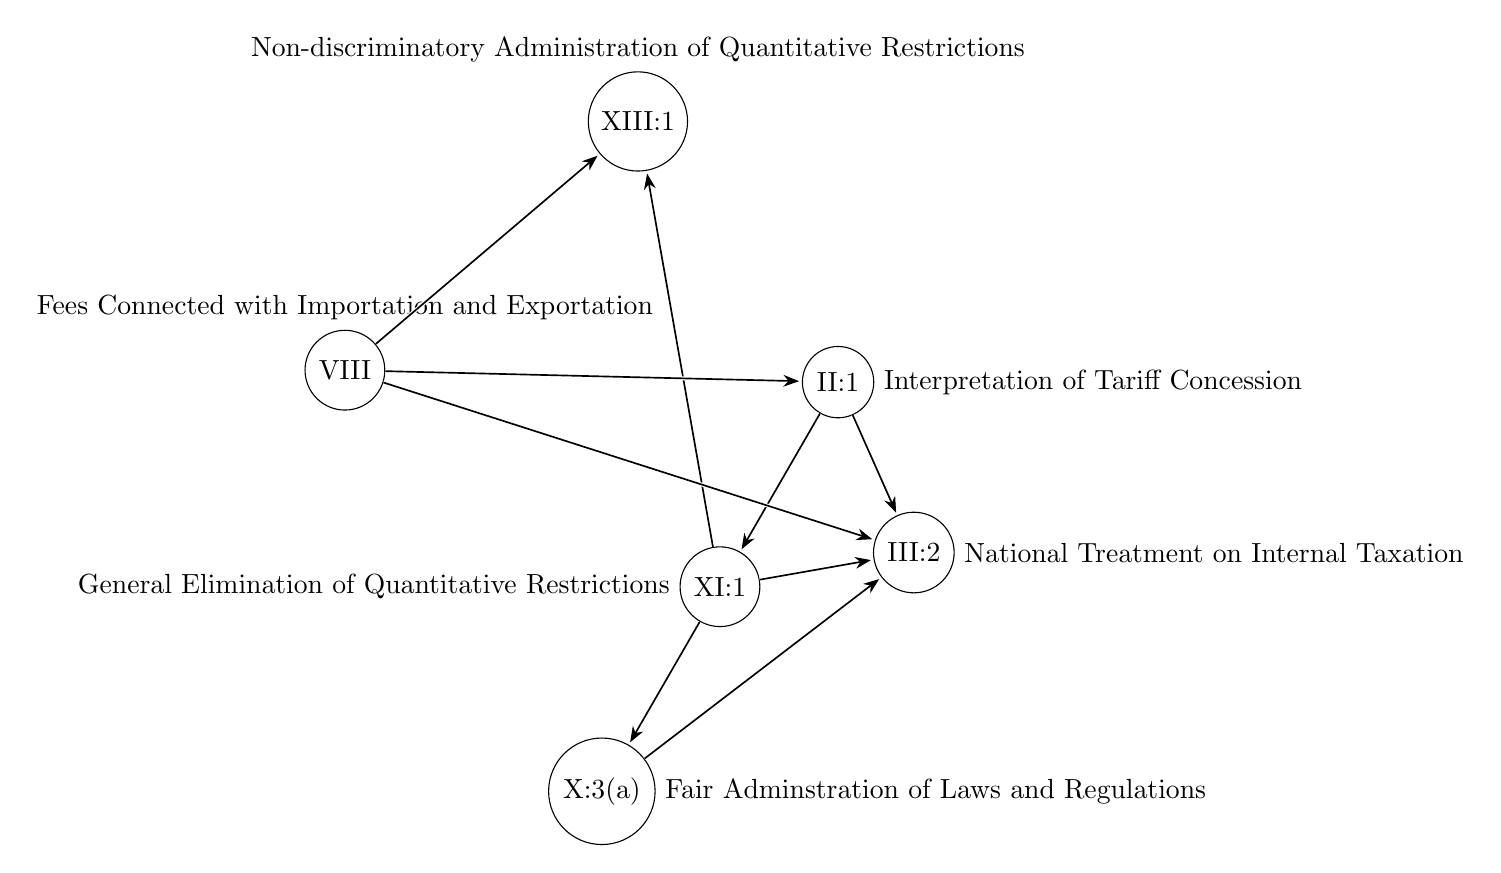
\begin{tikzpicture}[>={Stealth[color=black]},shorten >=1pt,node distance=2cm,on grid,initial/.style={}]
  \node[state, label=right:Interpretation of Tariff Concession] (T1) {II:1};
  \node[state, label=left:General Elimination of Quantitative Restrictions] at ([shift=({240:3 cm})]T1) (T4) {XI:1};
  \node[state, label=right:Fair Adminstration of Laws and Regulations] at ([shift=({240:3 cm})]T4) (T5) {X:3(a)};
  \node[state, label=above:Non-discriminatory Administration of Quantitative Restrictions] at ([shift=({100:6 cm})]T4) (T7) {XIII:1};
  \node[state, label=right:National Treatment on Internal Taxation] at ([shift=({10:2.5 cm})]T4) (T6) {III:2};
  \node[state, label=above:Fees Connected with Importation and Exportation] at ([shift=({150:5.5 cm})]T4) (T8) {VIII};

  \begin{scope}[every edge/.append style={->, double=black, draw=white}] % for directed edge, change "style={->, double=black, draw=white}]"
    \path (T1)
    edge   (T4)
    edge   (T6);
    \path (T4)
    edge   (T5)
    edge   (T6)
    edge   (T7);
    \path (T5)
    edge   (T6);
    \path (T8)
    edge   (T7)
    edge   (T1)
    edge   (T6);

  \end{scope}
\end{tikzpicture}

% to draw the node's border w/ color, refer to https://tex.stackexchange.com/questions/438412/how-to-add-border-to-a-node
  }
  \caption{{\bf Network of the Articles of the WTO Agreement:} 
  This figure demonstrates a network of articles of WTO agreements
  that achieves \textit{Market Access} principle together.
  }
  \label{fig:market-aceess_directed}
\end{figure}

\section{Data}

\begin{itemize}
  \item exemplify as detail as possible to inform readers about how data looks like.
  \item Privide a running example that shows how WTO works with data. 
  \item (Borrow from the previous paper)
  
\end{itemize}

\section{Methodology}

\begin{itemize}
  \item Compare co-occurrences/neural network approach.

  \item Show that co-occurrences approach isn't accurate.
\end{itemize}

% == HEATMAP MATRIX == 
\begin{figure}[!tbp]
  \begin{subfigure}[b]{0.49\textwidth}
    \centering{
      \resizebox{\textwidth*\real{\heatmap}}{\textwidth*\real{\heatmap} * \real{1.7889}}{% This file was created by tikzplotlib v0.9.4.
\begin{tikzpicture}

\begin{axis}[
hide x axis,
hide y axis,
tick align=outside,
tick pos=left,
x grid style={white!69.0196078431373!black},
xmin=0, xmax=80,
xtick style={color=black},
y grid style={white!69.0196078431373!black},
ymin=0, ymax=143,
ytick style={color=black}
]
\addplot graphics [includegraphics cmd=\pgfimage,xmin=0, xmax=80, ymin=0, ymax=143] {co-citation-004.png};
\end{axis}

\end{tikzpicture}
}
      \caption{Co-citation Matrix}
      \label{sparse_matrix}
    }
  \end{subfigure}
  \hfill
  \begin{subfigure}[b]{0.49\textwidth}
    \centering{
      \resizebox{\textwidth*\real{\heatmap}}{\textwidth*\real{\heatmap} * \real{1.7889}}{% This file was created by tikzplotlib v0.9.4.
\begin{tikzpicture}

\begin{axis}[
hide x axis,
hide y axis,
tick align=outside,
tick pos=left,
x grid style={white!69.0196078431373!black},
xmin=0, xmax=80,
xtick style={color=black},
y grid style={white!69.0196078431373!black},
ymin=0, ymax=143,
ytick style={color=black}
]
\addplot graphics [includegraphics cmd=\pgfimage,xmin=0, xmax=80, ymin=0, ymax=143] {pred_only.png};
\end{axis}

\end{tikzpicture}
}
      \caption{Prediction Matrix}
      \label{predidction_matrix}
    }
  \end{subfigure}
  \caption{{\bf Spare \& Dense Representation}}
  \label{sparse_dense}
\end{figure}


\section{Empirical Findings}
No Greeks. English. Three Networks.

% == THREE SUBSYSTEM == 
\begin{figure}
  \centering{
    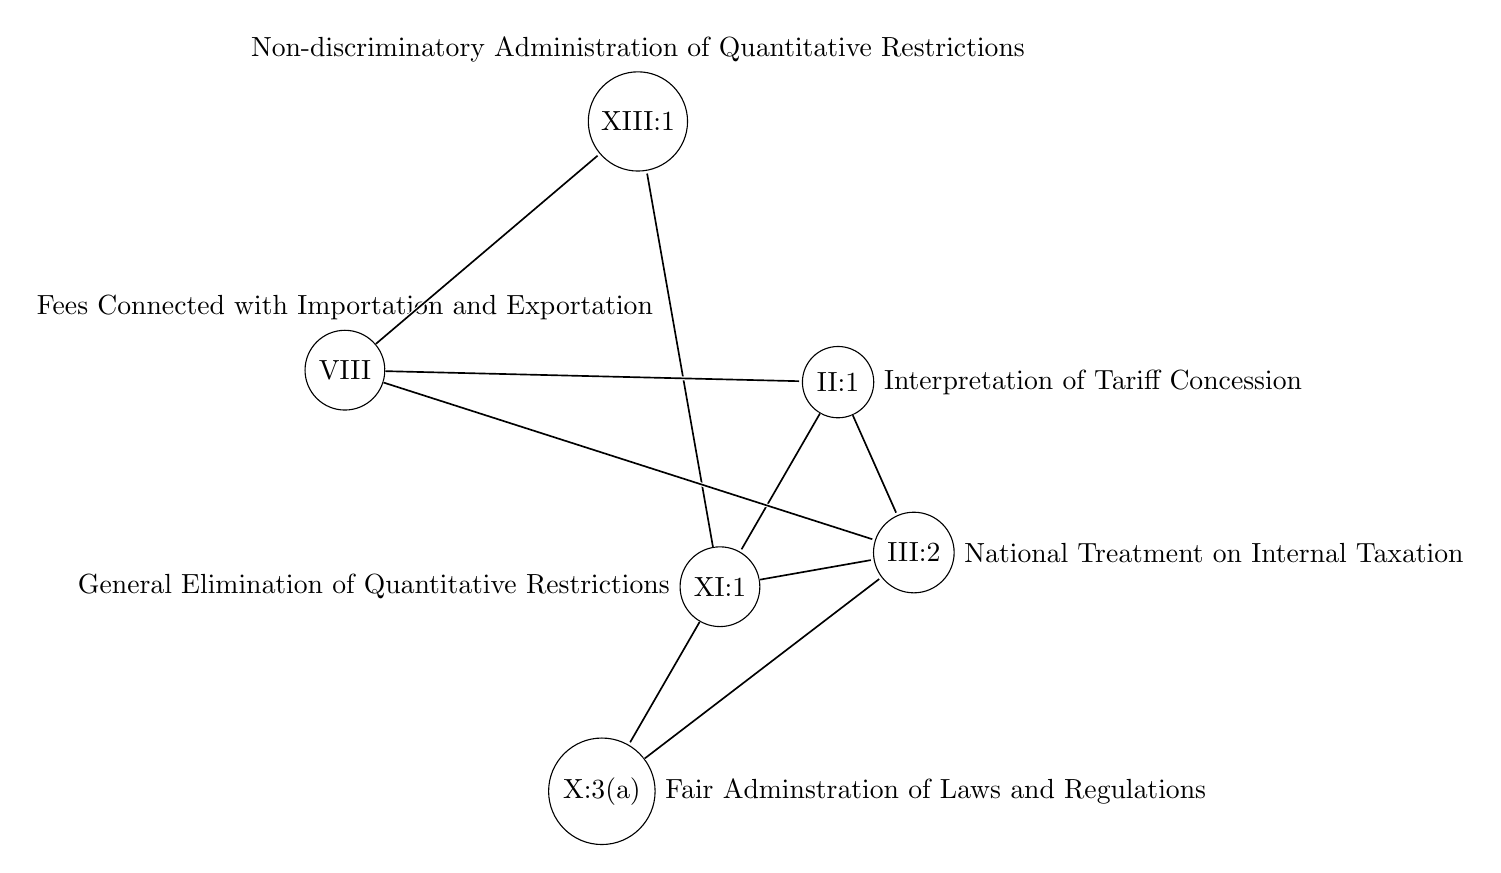
\begin{tikzpicture}[>={Stealth[color=black]},shorten >=1pt,node distance=2cm,on grid,initial/.style={}]
  \node[state, label=right:Interpretation of Tariff Concession] (T1) {II:1};
  \node[state, label=left:General Elimination of Quantitative Restrictions] at ([shift=({240:3 cm})]T1) (T4) {XI:1};
  \node[state, label=right:Fair Adminstration of Laws and Regulations] at ([shift=({240:3 cm})]T4) (T5) {X:3(a)};
  \node[state, label=above:Non-discriminatory Administration of Quantitative Restrictions] at ([shift=({100:6 cm})]T4) (T7) {XIII:1};
  \node[state, label=right:National Treatment on Internal Taxation] at ([shift=({10:2.5 cm})]T4) (T6) {III:2};
  \node[state, label=above:Fees Connected with Importation and Exportation] at ([shift=({150:5.5 cm})]T4) (T8) {VIII};

  \begin{scope}[every edge/.append style={-, double=black, draw=white}] % for directed edge, change "style={->, double=black, draw=white}]"
    \path (T1)
    edge   (T4)
    edge   (T6);
    \path (T4)
    edge   (T5)
    edge   (T6)
    edge   (T7);
    \path (T5)
    edge   (T6);
    \path (T8)
    edge   (T7)
    edge   (T1)
    edge   (T6);

  \end{scope}
\end{tikzpicture}

% to draw the node's border w/ color, refer to https://tex.stackexchange.com/questions/438412/how-to-add-border-to-a-node
  }
  \caption{Market Access}
  \label{fig:market-aceess}
\end{figure}




\section{Conclusion}
This paper shows how WTO works.

\begin{itemize}
  \item Implicaiton of thie method in general.
  \item Address the imbalance of legal capacity between developed/ing countries
\end{itemize}

\clearpage

\bibliography{bibtemplate}

\section{Appendix}

\begin{displayquote}[][]
  \begin{center}
    Article 7\\
    Terms of Reference of Panels
  \end{center}

  1. Panels shall have the following terms of reference unless the parties to the dispute
  agree otherwise within 20 days from the establishment of the panel:

  \begin{displayquote}[][]

    ``To examine, in the light of {\bf the relevant provisions} in (name of the covered
    agreement(s) cited by the parties to the dispute), the matter referred to the DSB by
    (name of party) in document … and to make such findings as will assist the DSB in
    making the recommendations or in giving the rulings provided for in that/those
    agreement(s).''
      
  \end{displayquote}

  2. Panels shall address {\bf the relevant provisions} in any covered agreement or agreements
  cited by the parties to the dispute.

  \ldots
\end{displayquote}

% == END
\end{document}